\documentclass[../DoAn.tex]{subfiles}
\begin{document}

Trong đồ án tốt nghiệp này, em đã tìm hiểu và triển khai thực tế hai phần kiến thức khó và mới mẻ đó là kiến trúc Microservice
và giao thức OAuth2 trong lĩnh vực xây dựng phần mềm doanh nghiệp. Dưới đây, em sẽ trình bày chi tiết về những lý thuyết đã tìm hiểu được
và áp dụng vào thực hành xây dựng sản phẩm cho đồ án tốt nghiệp này.

\section{Ứng dụng kiến trúc Microservice trong phát triển phần mềm}
\label{section:5.1}

\subsection{Đặt vấn đề}
\label{subsection:5.1.1}
Trong quá trình tìm hiểu bài toán đặt ra, em nhận thấy hệ thống sau khi triển khai sẽ cần cùng lúc đảm nhiệm nhiều nhóm chức năng khác nhau,
ví dụ như nhóm chức năng về quản lý người dùng và thông tin cá nhân của họ, nhóm chức năng về kết nối và quản lý một hệ thống gửi thư điện tử bên ngoài
hệ thống chính, nhóm chức năng về theo dõi các phiên đăng nhập, người dùng trực tuyến để gửi thông báo cho họ, hay
nhóm chức năng về thực hiện các công việc đã được hẹn giờ hoặc lặp đi lặp lại nhiều lần trong ngày.

Với những yêu cầu kỹ thuật khác nhau như vậy, việc xây dựng hệ thống sử dụng một máy chủ duy nhất (kiến trúc Monolith) sẽ gặp nhiều khó khăn.
Ví dụ, các chức năng sử dụng các công việc hẹn giờ trước hay lặp đi lặp lại nhiều lần trong ngày sẽ cần một máy chủ chạy liên tục. Nếu có lỗi phát sinh,
cơ chế tự khôi phục lỗi của máy chủ cần được cài đặt nhưng phải đảm bảo được các công việc đã lập lịch phải được sao lưu lại.
Tương tự như vậy, chức năng theo dõi người dùng trực tuyến và gửi thông báo cũng yêu cầu máy chủ sẽ phải chạy liên tục và quản lý số lượng lớn
các kết nối Websocket. Điều này sẽ làm tăng đáng kể chi phí về phần cứng và chi phí vận hành hệ thống. Ngoài ra, việc phát sinh lỗi và tự động khôi phục
của các chức năng có thể làm ảnh hưởng lẫn nhau, gây ra mất mát dữ liệu trong khi vận hành.

Ngoài các chức năng về kỹ thuật như trên, nghiệp vụ của hệ thống cũng có các nhóm riêng biệt, ví dụ như nhóm chức năng về quản lý công việc,
nhóm chức năng về quản lý đội, tổ chức, nhóm chức năng về báo cáo và thống kê. Ví dụ, người dùng có thể chỉ cần sử dụng chức năng để tạo báo cáo
và xem thống kê các thông số của dự án và không cần các chức năng khác. Nếu có nhiều người dùng như vậy, họ sẽ làm tăng tải chung cho hệ thống và
cách khắc phục duy nhất là gia tăng phần cứng kèm theo chi phí vận hành. Trong đó có bao gồm những chức năng ít được sử dụng hơn sẽ gây lãng phí.

Sau quá trình tìm hiểu về các kiến trúc phần mềm hiện đại, em nhận thấy kiến trúc Microservices là một giải pháp phù hợp với bài toán đặt ra.
Nguyên lý chia nhỏ hệ thống thành các dịch vụ nhỏ, độc lập với nhau như đã trình bày ở phần \ref{section:4.1} sẽ giúp giải quyết được các vấn đề
trên.

\subsection{Giải pháp}
\label{subsection:5.1.2}

Như đã trình bày trong phần \ref{section:4.1}, Microservices là một kiến trúc phần mềm mà trong đó một ứng dụng được xây dựng thành nhiều dịch vụ nhỏ,
chúng được mô hình hoá xoay quanh những nhóm nghiệp vụ cụ thể. Thật vậy, không phải mọi hệ thống đều cần phải sử dụng kiến trúc Microservices,
việc quyết định sử dụng kiến trúc nào phải dựa trên nghiệp vụ của toàn bộ dự án. Nếu nghiệp vụ của dự án có tính độc lập cao, các nhóm nghiệp vụ
không phụ thuộc nhiều vào nhau, thì kiến trúc Microservice là một lựa chọn tốt để triển khai về đường dài.

Đầu tiên, để triển khai một hệ thống theo kiến trúc Microservice, nhà phát triển phần mềm sẽ cần xây dựng một cơ sở hạ tầng kỹ thuật đủ tốt bên dưới
để hỗ trợ cho việc triển khai nghiệp vụ sau này. Do hệ thống cần được chia nhỏ và chạy độc lập với nhau, việc bao đóng
các thành phần này cần đảm bảo rằng mã nguồn của của chúng có thể chạy ổn định và giống nhau ở mọi môi trường. Như đã trình bày ở phần \ref{section:3.1} và
\ref{section:3.2}, em quyết định sử dụng Docker và Kubernetes để đóng gói các thành phần của mã nguồn, do là hai công nghệ này đang phổ biến nhất hiện nay
để xây dựng một cơ sở hạ tầng hỗ trợ cho việc triển khai kiến trúc Microservices. Với Docker, mỗi thành phần sẽ có một tệp tin Dockerfile riêng,
bên trong đó chứa định nghĩa của các bước từ mã nguồn có thể xây dựng thành một "container", trong đó bao gồm cả các thư viện cần thiết,
câu lệnh để xây dựng và triển khai. Quá trình trên sẽ tạo ra một bản thiết kế "container", chúng được gọi là Docker Image, thành phần này cần được
đưa lên một kho lưu trữ trực tuyến để các dịch vụ máy chủ có thể truy cập. Sau đó, em sử dụng Kubernetes để tải các Docker Image này về
và triển khai từng phần lên máy chủ vật lý. Các tính năng chính của Kubernetes em đã trình bày ở phần \ref{section:3.2}, tuy nhiên mỗi dịch vụ của hệ thống đều có yêu cầu riêng
về cấu hình phần cứng, cách thức kết nối nội bộ và kết nối với Internet. Dó đó, em sử dụng Helm, là một công nghệ chuẩn hoá các thành phần trong Kubernetes,
để đóng gói các cấu hình này thành một bản thiết kế riêng, dưới dạng tệp tin có đuôi .yaml. Như vậy, khi triển khai một dịch vụ, em sẽ viết các tệp tin cấu hình theo một cấu trúc
nhất định, sau đó sử dụng Helm để đóng gói và triển khai lên Kubernetes. Hơn nữa em có thể thay đổi các cấu hình này ngay trong quá trình vận hành mà không bị gián đoạn hay tái triển khai
lại mã nguồn. Đối với các thành phần không xây dựng từ mã nguồn, ví dụ như cơ sở dữ liệu hay hàng đợi tin nhắn, Helm cũng cung cấp các tệp tin cấu hình có sẵn, em sẽ sửa đổi theo nhu cầu
thực tế.

\begin{figure}[H]
    \centering
    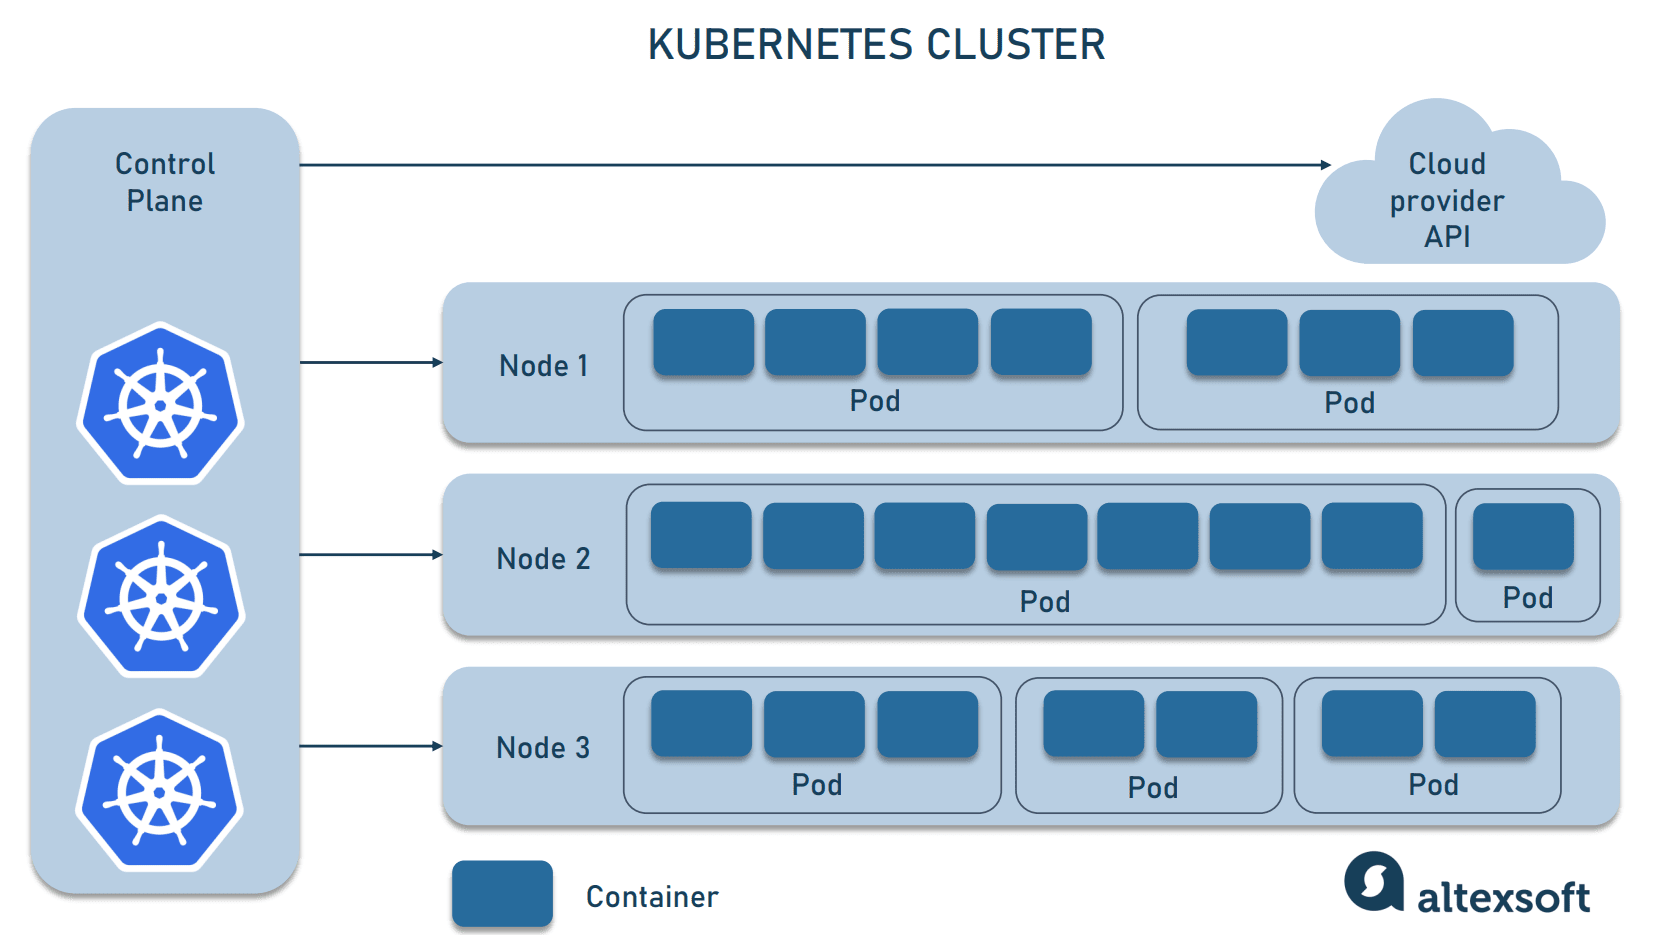
\includegraphics[width=1.0\linewidth]{Hinhve/Example_Kubernetes.png}
    \caption{Minh hoạ các thành phần của hệ thống sau khi triển khai lên Kubernetes (Nguồn: AltexSoft)}
    \label{fig:Example_Kubernetes}
\end{figure}

Trong hình minh hoạ, mỗi "Container" nằm trong một "Pod", Pod tương ứng với một dịch vụ của hệ thống, cơ chế tự nhân lên khi gặp tải cao về cơ bản là Pod sẽ sao chép
Container bên trong nó để chạy song song với nhau. Mỗi Pod sẽ nằm trong một "Node", Node là một máy chủ vật lý, có thể là máy chủ ảo hoặc máy chủ vật lý thực, Node cũng có cơ chế tự sao chép chính nó
để nhân lên. Các máy chủ này cùng với các thành phần quản lý của Kubernetes sẽ tạo thành một cụm máy chủ, được gọi là "Cluster". Để dễ dàng quản lý toàn bộ hệ thống, em quyết định
sử dụng dịch vụ Kubernetes của Google Cloud Platform để vận hành trên máy chủ vật lý, tên là Google Kubernetes Engine.

Sau quá trình trên, tuy việc quản lý vận hành đã được tự động hoá, nhưng mọi bước triển khai vẫn phải thực hiện thủ công nếu có thay đổi ở mã nguồn. Mặt khác,
do việc phát triển vẫn diễn ra liên tục sau khi hệ thống được triển khai, các thay đổi thường xuyên xảy ra là điều tất yếu. Do đó, em đã xây dựng một quy trình tự động hoá triển khai mã nguồn
khi có thay đổi. Do mã nguồn được lưu trữ trên Github, em sử dụng Github Action để tự động triển khai mã nguồn ở Google Kubernetes Engine. Cụ thể, em đã viết một tệp tin cấu hình cho mỗi dịch vụ,
trong đó chứa các bước để tự động thực hiện lại toàn bộ quy trình triển khai ở trên, bao gồm kiểm tra lỗi trong mã nguồn, xây dựng thành Docker Image, đẩy lên kho lưu trữ ở Google Cloud,
thực thi các lệnh để triển khai lên Google Kubernetes Engine.Như vậy, thời gian và công sức của các nhà phát triển sẽ được giảm bớt đáng kể, đồng thời giảm thiểu
các lỗi phát sinh trong quá trình triển khai, lợi ích này càng tăng lên nếu thời gian thực hiện dự án càng dài. Ngoài ra, quá trình này có thể tích hợp thêm
các bước kiểm thử tự động, kiểm tra bảo mật cho mã nguồn, giúp đảm bảo chất lượng của các lần thay đổi không sinh ra các lỗi cơ bản.

Bên trong một hệ thống Microservice, các dịch vụ tuy chạy độc lập với nhau, song, với một số nghiệp vụ cần nhiều dữ liệu hơn một dịch vụ có thể đáp ứng, việc giao tiếp
giữ các dịch vụ là điều cần thiết. Trong đó bao gồm một phương thức giao tiếp đồng bộ là gọi hàm từ xa của Google (Google Remote Procedure Call - gRPC) và một phương thức giao tiếp bất đồng bộ là
hàng đợi tin nhắn (Message Queue). Với gRPC, em cần định nghĩa các giao diện dịch vụ bằng ngôn ngữ Protocol Buffer, sau đó sử dụng công cụ của Google để sinh ra mã nguồn từ giao diện đó.
Từ các lớp và phương thức được sinh ra, các dịch vụ có thể giao tiếp với nhau một cách nhanh chóng hơn các giao thức phổ biến khác như HTTP. Điều này là do thông điệp
được gửi qua gRPC sẽ được mã hóa dưới dạng nhị phân, giúp giảm thiểu kích thước gói tin và tăng tốc độ truyền tải. Đối với hàng đợi tin nhắn, em sử dụng RabbitMQ để triển khai,
và Masstransit để trừu tượng hoá cấu hình, câu lệnh điều khiển của RabbitMQ dưới dạng mã nguồn C\# (ngôn ngữ lập trình chính của hệ thống back-end). Do đây là một giao thức bất đồng bộ,
các dịch vụ không cần thiết phải chờ đợi nhau mà có thể gửi và nhận thông điệp một cách độc lập. Điều này giúp tăng tốc độ xử lý của hệ thống, tuy vậy, giao thức này yêu cầu
hàng đợi tin nhắn phải đủ tin cậy và có cơ chế an toàn tránh mất mát dữ liệu.

\begin{figure}[H]
    \centering
    \includegraphics[width=1.0\linewidth]{Hinhve/Example_RabbitMQ.png}
    \caption{Minh hoạ phương thức giao tiếp bằng hàng đợi tin nhắn trong kiến trúc Microservices (Nguồn: Microsoft)}
    \label{fig:Example_Kubernetes}
\end{figure}

\newpage

\subsection{Kết quả đạt được}
\label{subsection:5.1.3}

Sau khi thực hiện triển khai giải pháp nếu trên, hệ thống hiện tại đang có 10 ứng dụng nhỏ chạy độc lập với nhau, trong đó có 5 dịch vụ chính thực hiện nghiệp vụ,
và các thành phần hỗ trợ như cơ sở dữ liệu, bộ nhớ tạm, hàng đợi tin nhắn. Tất cả các thành phần này đều trong trạng thái hoạt động ổn định và được theo dõi hoạt động
kiểm soát tài nguyên tiêu thụ.

\begin{figure}[H]
    \centering
    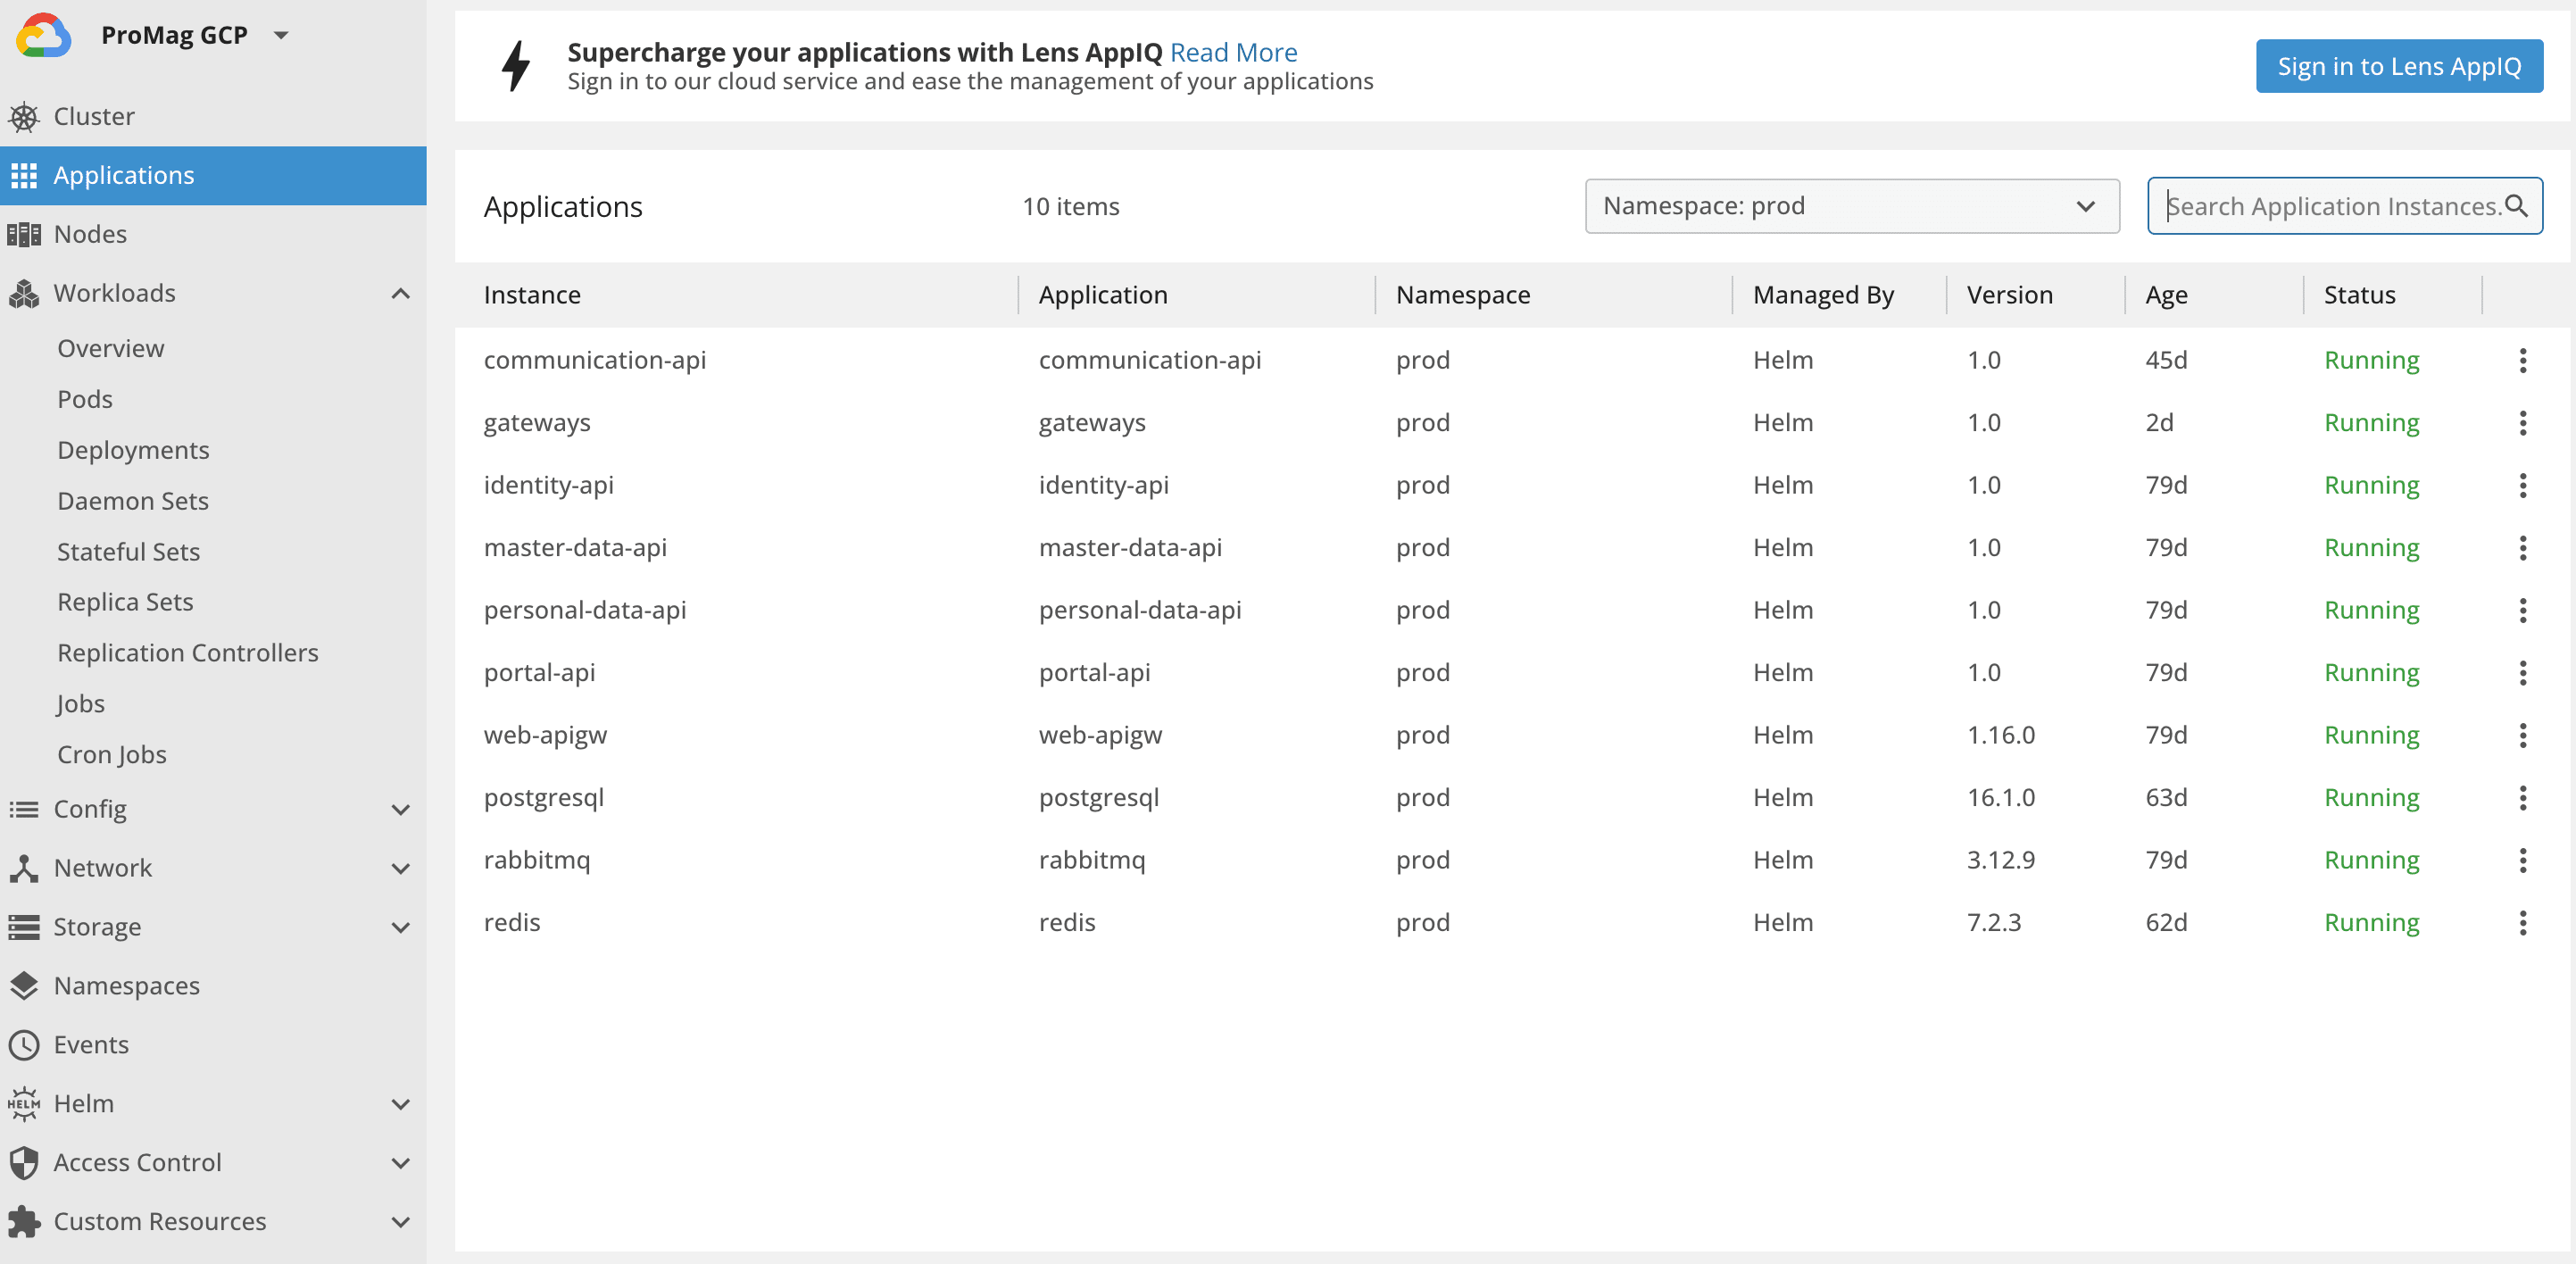
\includegraphics[width=1.0\linewidth]{Hinhve/Result_Lens.png}
    \caption{Các thành phần trong hệ thống sau khi triển khai lên Kubernetes}
    \label{fig:Result_Lens}
\end{figure}

\begin{figure}[H]
    \centering
    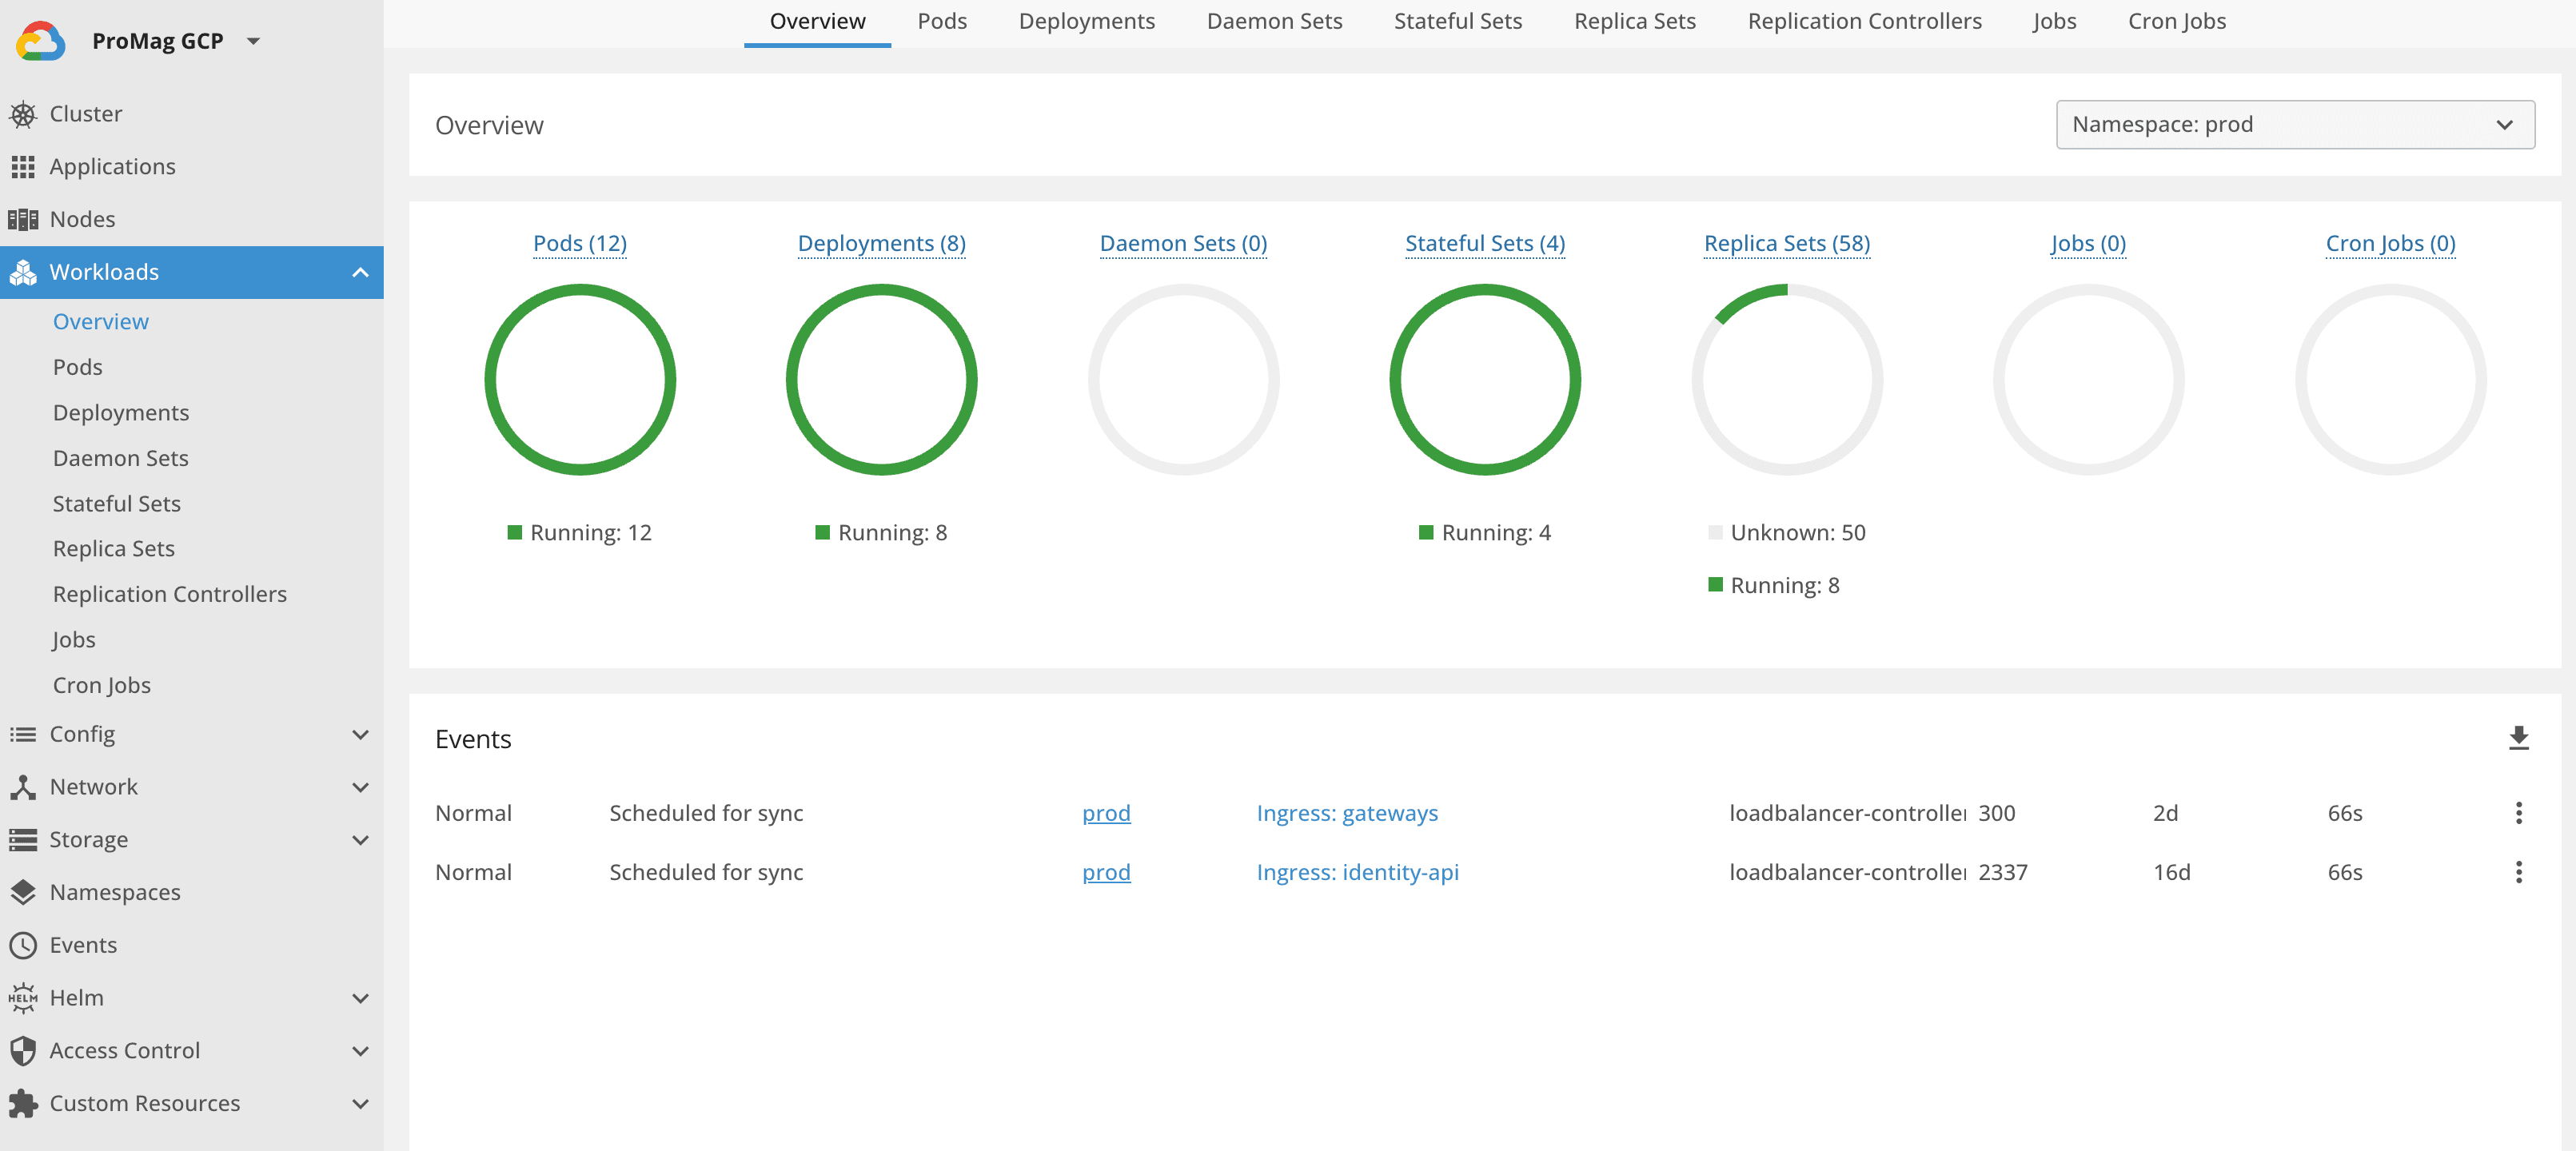
\includegraphics[width=1.0\linewidth]{Hinhve/Result_Lens_Status.png}
    \caption{Trạng thái hệ thống sau khi triển khai lên Kubernetes}
    \label{fig:Result_Lens_Status}
\end{figure}

\newpage

Các thành phần này đều được tự động tích hợp và triển khai bằng Github Actions, trong đó, em đã cấu hình 14 luồng triển khai tự động cho mọi thành phần trong hệ thống,
bảo gồm các các dịch vụ chính, các thành phần hỗ trợ vận hành cũng như các công cụ hỗ trợ phát triển. Toàn bộ các luồng triển khai này đã được tự động chạy 293 lần,
tương ứng với 293 lần thay đổi mã nguồn được đẩy lên kho lưu trữ Github. Các luồng này nếu gặp lỗi đều được thông báo qua thư điện tử, chỉ trường hợp này,
em mới cần phải can thiệp thủ công để khắc phục lỗi. Như vậy, việc triển khai mã nguồn đã được tự động hoá, giúp tiết kiệm thời gian và công sức của các nhà phát triển
tăng dần hiệu quả theo thời gian.

\begin{figure}[H]
    \centering
    \includegraphics[width=1.0\linewidth]{Hinhve/Result_GithubAction.png}
    \caption{Các luồng triển khai tự động bằng Github Actions}
    \label{fig:Result_GithubAction}
\end{figure}

\newpage

\section{Ứng dụng giao thức OAuth2 trong xác thực và phân quyền người dùng}
\label{section:5.2}

\subsection{Đặt vấn đề}
\label{subsection:5.2.1}

Trong quá trình tìm hiểu bài toán đề tài đặt ra, em nhận thấy mọi hệ thống phần mềm đều cần phải có một cơ chế xác thực và phân quyền người dùng để đảm bảo tính bảo mật
của hệ thống nói chung và dữ liệu cá nhân của người dùng nói riêng. Đối với các hệ thống truyền thống, việc xác thực và phân quyền người dùng thường được thực hiện
ngay trên chính hệ thống back-end của nó dươi một số dạng phổ biến như xác thực bằng tài khoản và mật khẩu, xác thực bằng mã xác thực một lần (OTP), xác thực bằng
Token. Vấn đề của cách triển khai này là mỗi hệ thống phải tự xây dựng cơ chế xác thực riêng, phải xử lý các vấn đề liên quan đến bảo mật, mã hoá thông tin.
Nếu hệ thống có nhiều ứng dụng khác nhau cùng truy cập, với mỗi nhu cầu khác nhau, hệ thống bắt buộc phải xây dựng thêm các tính năng dành cho nhu cầu của ứng dụng đó,
gây lãng phí về thời gian và công sức. Mặt khác, nếu nhà phát triển xây dựng một phần back-end riêng cho mỗi ứng dụng, họ sẽ phải lặp lại quá trình xây dựng cơ chế xác thực và phân quyền.
Ngoài ra, nguy cơ bị nghe lén thông tin trên đường truyền cũng có thể xảy ra, do đối tượng đã nhắm vào hệ thống từ trước.

Với các vấn đề trên, em nhận thấy việc xây dựng một hệ thống xác thực và phân quyền người dùng riêng biệt, có thể được sử dụng cho nhiều ứng dụng khác nhau là một giải pháp tốt.
Điều này sẽ giúp giảm thiểu thời gian và công sức xây dựng, đồng thời giảm thiểu các lỗi phát sinh trong quá trình xây dựng. Lợi ích này sẽ được tăng theo thời gian nếu như
hệ thống được sử dụng cho càng nhiều ứng dụng khác nhau.

Hơn nữa, cơ chế xác thực và phân quyền người dùng này có thể phục vụ cho các ứng dụng không hề cần sử dụng các hệ thống backend đằng sau mà chỉ cần thông tin
cơ bản của người dùng như tên, email, ảnh đại diện. Như vậy, người dùng chỉ cần lưu lại thông tin cá nhân ở một nơi, và có thể cấp quyền cho các ứng dụng khác
truy cập vào chúng. Tất nhiên những quyền này cũng cần phải được thu hồi nếu người dùng không muốn sử dụng ứng dụng đó nữa.

\subsection{Giải pháp}
\label{subsection:5.2.2}

Sau khi tìm kiếm các giải pháp các khác nhau cho vấn đề này, em nhận thấy giao thức OAuth2 là một đáp án phù hợp nhất. OAuth2 là một giao thức ủy quyền, được sử dụng
để xác thực và phân quyền người dùng cho các ứng dụng khác nhau. Về cơ bản, OAuth2 đưa ra một tiêu chuẩn bảo mật của sự việc: người dùng cấp quyền cho một ứng dụng
truy cập vào thông tin cá nhân của họ đang nằm trên một ứng dụng khác. Ví dụ, sau khi em đăng ký một tài khoản trên GitHub, thông tin cá nhân của em đã được lưu trữ lại
trên máy chủ của GitHub. Sau đó, em có sử dụng một ứng dụng khác là LeetCode, để đăng nhập vào LeetCode, em có thể sử dụng tài khoản GitHub của mình. Để làm điều này,
em sẽ phải cấp quyền cho LeetCode truy cập vào các thông tin cần thiết từ máy chủ của GitHub. Quá trình ba bên này cần thiết phải được diễn một cách an toàn và bảo mật.

Trước hết, để hiểu rõ hơn về cơ chế hoạt động của OAuth2, em sẽ trình bày một số khái niệm cơ bản của giao thức này. Quá trình trình xác thực ba bên này bao gồm
người dùng (User), ứng dụng khách (Client) và máy chủ xác thực (Authorization Server). Trong đó, người dùng là người sử dụng ứng dụng, Client là ứng dụng mà người dùng
muốn truy cập, Authorization Server là máy chủ chứa thông tin người dùng và cấp quyền cho Client. Với một số hệ thống lớn, Authorization Server chỉ đảm nhận công việc xác thực,
dữ liệu cá nhân của người dùng được lưu ở Resource Server. Tuy nhiên, trong trường hợp của đồ án tốt nghiệp này, em sẽ sử dụng cả hai chức năng trên một máy chủ duy nhất.

Trước khi quá trình xác thực và cấp quyền diễn ra, Client cần phải đăng ký với Authorization Server, thông qua đó, Client sẽ nhận được một mã định danh (Client ID)
và một chuỗi bí mật (Client Secret). Khi User muốn truy cập vào Client, Client sẽ yêu cầu User cấp quyền truy cập vào thông tin cá nhân của họ. Nếu User đồng ý, Client sẽ gửi
yêu cầu này đến Authorization Server, kèm theo mã định danh và chuỗi bí mật của mình. Sau đó, một chuỗi các bước xác thực diễn ra giữa Client và Authorization Server,
và cuối cùng, Client sẽ nhận được một mã truy cập (Access Token) và một mã làm mới (Refresh Token). Mã truy cập này sẽ được Client sử dụng để truy cập vào thông tin cá nhân của User,
còn mã làm mới sẽ được Client sử dụng để làm mới mã truy cập khi nó hết hạn. Mã truy cập này sẽ được gửi kèm theo mỗi yêu cầu từ Client đến Authorization Server, để máy chủ có thể xác thực.

Tuy vậy, định nghĩa và nội dung của OAuth2 chỉ nằm trên lý thuyết, để triển khai thực tế, em sẽ sử dụng một lớp trừu tượng hoá của OAuth2, đó là OpenID Connect (OIDC).
OIDC là một giao thức xác thực và phân quyền người dùng, được xây dựng dựa trên OAuth2. OIDC định nghĩa thêm một số khái niệm và quy trình mới, giúp việc triển khai
thực tế dễ dàng hơn. Trong đó, OIDC định nghĩa thêm một khái niệm mới là ID Token, đây là một mã thông báo chứa thông tin cá nhân của User, được mã hoá bằng JSON Web Token (JWT).

\newpage

\subsection{Kết quả đạt được}
\label{subsection:5.2.3}

Sau khi thực hiện triển khai giải pháp trên, hệ thống hiện tại đã có một cơ chế xác thực và phân quyền người dùng riêng biệt, có thể được sử dụng cho nhiều ứng dụng khác nhau.
Máy chủ xác thực này được triển khai riêng so với các dịch vụ khác trong hệ thống back-end, với máy chủ ảo và đặt tên miền riêng biệt. Sau khi người dùng đã đăng nhập vào máy chủ xác thực,
đối với người dùng mới của ứng dụng Web, họ sẽ được yêu cầu cung cấp các quyền truy cập tới thông tin cá nhân của họ, cũng như truy cập vào các
dịch vụ cần thiết cho ứng dụng. Sau khi đồng ý, họ sẽ được chuyển hướng về ứng dụng Web, và có thể sử dụng các chức năng của ứng dụng bình thường.

\begin{figure}[H]
    \centering
    \includegraphics[width=1.0\linewidth]{Hinhve/Screenshot_AcceptAccess.png}
    \caption{Minh hoạ yêu cầu cung cấp quyền truy cập đối cho người dùng mới}
    \label{fig:Result_GithubAction}
\end{figure}

\newpage

\end{document}